\documentclass[journal, a4paper]{IEEEtran}

% some very useful LaTeX packages include:



\usepackage{graphicx}   % Written by David Carlisle and Sebastian Rahtz
                        % Required if you want graphics, photos, etc.
                        % graphicx.sty is already installed on most LaTeX
                        % systems. The latest version and documentation can
                        % be obtained at:
                        % http://www.ctan.org/tex-archive/macros/latex/required/graphics/
                        % Another good source of documentation is "Using
                        % Imported Graphics in LaTeX2e" by Keith Reckdahl
                        % which can be found as esplatex.ps and epslatex.pdf
                        % at: http://www.ctan.org/tex-archive/info/


\usepackage{url}        % Written by Donald Arseneau
                        % Provides better support for handling and breaking
                        % URLs. url.sty is already installed on most LaTeX
                        % systems. The latest version can be obtained at:
                        % http://www.ctan.org/tex-archive/macros/latex/contrib/other/misc/
                        % Read the url.sty source comments for usage information.



\usepackage{amsmath}    % From the American Mathematical Society
                        % A popular package that provides many helpful commands
                        % for dealing with mathematics. Note that the AMSmath
                        % package sets \interdisplaylinepenalty to 10000 thus
                        % preventing page breaks from occurring within multiline
                        
\usepackage{float}


% Your document starts here!
\begin{document}

% Define document title and author
	\title{Independent Study Report}
	\author{Benjamin Gibbs\\ \vspace{.35cm} August 15, 2017 $\vert$ ASTR 4840-902\\ \vspace{.35cm} Advisor: Dr. Vladimir Zhdankin\\}
	\markboth{University of Colorado at Boulder}{}
	\maketitle


% Each section begins with a \section{title} command
\vspace{.4cm}
\section{Introduction}
\vspace{.4cm}
	% \PARstart{}{} creates a tall first letter for this first paragraph
	\PARstart{t}{his} report describes an independent study concerned with the analysis and visualization of a series of plasma turbulence simulations created by Vladimir Zhdankin and collaborators, and discussed in \textit{Kinetic Turbulence in Relativistic Plasma} \cite{zhdankin}. Of particular importance are the methods employed to access and manipulate simulation data, the theoretical background that separates the phenomenon of plasma turbulence from classical magnetohydrodynamic (MHD) turbulence, and the theoretical framework that both theories are built upon at the foundational level. In this report, pioneering measurements evaluated scale-dependent dynamic alignment in turbulent, relativistic plasma, the results of were qualitatively different from MHD simulations in the literature\cite{boldyrev}, pointing to the possibility of interesting new physics in the turbulent cascade for plasmas in this essentially unexplored regime. Additionally discussed are the significant structures observable from the visualizations of 'snapshots' of time evolved simulations and how bulk structures and trends can be related to the behavior of individual particles.

\vspace{.5cm}
\section{Methods and Background}
\vspace{.3cm}

The primary motivation for this independent study is the desire to pursue frontier research in physics that is accessible from an undergraduate level understanding. A personal interest in astrophysical science also influenced the selection of a study that investigates phenomena like stellar winds, astrophysical jets, and accretion disks. All of these interests are fulfilled by plasma turbulence research, which presents an opportunity to scrape at a remarkably fast moving field with extensive applications in theoretical and observational physics. Additionally,the desire to develop skills relevant to analysis of large data sets, especially involving coding and encrypted network navigation, provided a strong motivation for entering a field dominated by computational approach to data analysis. In order to adapt to this requirement, Matlab and Python were integral in both visual and numerical analysis of data, the result of which was a necessary increase in programming proficiency on the part of the student. Also beneficial was the development of skills needed to navigate Verus, the computer cluster used by the Uzdensky group for high performance simulation, as well as data manipulation and transfer. In particular, data was transferred by use of unix commands 'ssh' and 'scp', both of which are concerned with the encryption of data systems and their contents.

Once in possession of a dataset transferred from the Verus system, analysis beyond basic visualizations required a stronger theoretical background in plasma turbulence. To serve this purpose, the independent study was accompanied by readings and discussion from Biskamp’s \textit{MHD Turbulence}\cite{biskamp}. The concepts most frequently addressed were the MHD equations defining the fundamental behavior of ionized fluids, the disturbance of said fluids and the subsequent behavior of turbulent fluid bodies.

The data which this report is concerned with is a particle in cell (PIC) simulation of a collisionless, relativistically hot, magnetized pair plasma body. Unless specified otherwise, the data under discussion is from one 'snapshot' of a $256^3$ cell simulation\cite{zhdankin}. For the purpose of this report, turbulence within said snapshot is treated as the phenomenon by which a disturbance of a laminar flow leads to the dissipation of kinetic energy in successively smaller 'eddies' of fluid motion. The assumption is made that across the inertial range the energy cascade rate is constant, or scale invariant.

 Following these establishments, the distinctions between classical MHD turbulence and the plasma turbulence involved in the simulations were then expanded on. Mny previous studies based on the MHD model use the momentum equation, shown below \ref{equation1}.
\vspace{.5cm}
\begin{equation}
\rho(\frac{\partial}{\partial t}+\vec{V} \cdotp \nabla)\vec{V}=\frac{\vec{J} \times \vec{B}}{c}-\nabla p
\label{equation1}
\end{equation}
\vspace{.3cm}

Note that in the preceding equation, $\rho$ is the fluid mass density, $\vec{V}$ is the fluid velocity, $c$ is the speed of light. Also $\vec{J}$, $\vec{B}$, and $-\nabla p$ are the current density, magnetic field, and pressure gradient, respectively. Additionally, Maxwell's equation for the magnetic field $\vec{B}$ needs to be solved in addition to the above equation in order to obtain a complete solution. Instead of the MHD model, the simulations we consider will be more fully described by the Lorentz force, shown below with $\vec{E}$ indicating the electric field [Equation \eqref{equation2}] and the sign of the expression being determined by the charge of the particle species in question. The expression is used to evolve a large number of particles that constitute the plasma body.

\vspace{.3cm}
\begin{equation}
\frac{d\vec{p}_i}{dt}=\pm e(\vec{E}+\frac{\vec{v}_i}{c} \times \vec{B})
\label{equation2}
\end{equation}
\vspace{.3cm}

In the above expression $ \vec{v}_i$ is the particle velocity. The Lorentz force above describes the first principle's interactions of the particles and is therefore more fundamental than the MHD model which is derived with many more assumptions than the above equation. Consequently an intuitive sense of system behavior can be obtained from the electromagnetic behavior, and the velocity of a system. To investigate this, visualizations of the system related to these parameters were made.

\vspace{.4cm}
\section{Visualizations}
\vspace{.4cm}

Having determined from the Lorentz equations that the primary objects used to describe the turbulent plasma systems are the velocities and electromagnetic projections of the charges described by the simulation, it follows that the most relevant depiction of the simulations should be as follows [Fig. \ref{figure1}]. Below, Fig. 1 shows the magnetic field of a 1cm thick layer at the surface of a simulation cube which spans $256^3$ cells [Fig. \ref{figure1}]. The thickness of the layer is determined by cell size, with each cell face spanning $1 cm$ of space, placing an effective parameter on slice volume. 
\vspace{.4cm}

\begin{figure}[H]
\caption{Contour Plot of Magnetic Field Magnitude at Simulation 'Slice'}
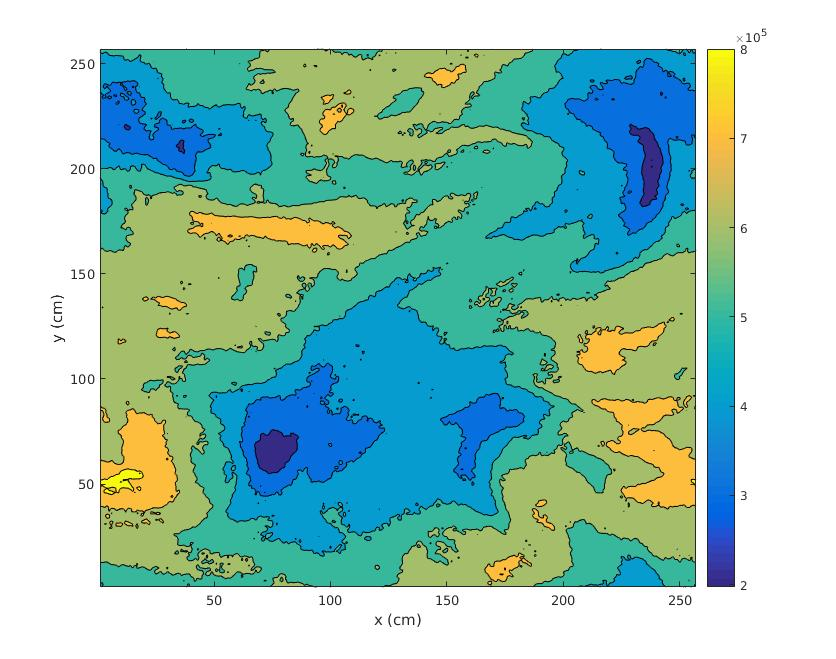
\includegraphics[width=9.5cm]{bfieldslice.jpg}
\label{figure1}
\centering
\end{figure}
\vspace{.4cm}

The magnetic field was selected for representation of all electromagnetic behavior because of its visual similarity to the electric field, which was verified through renderings of electric field contour plots similar to this one. Because of its relationship to dynamic alignment (outlined in the following section), the magnetic field is the most relevant of the two fields for display. Notable in the above figure are the high magnitude regions which indicate a sheet-like structure which results from dissipative trends in the particle bulk. Similar sheet-like structures can be seen in the following contour plot [Fig. \ref{figure2}] of current density $\vec{J}$. The following figure was selected to visually demonstrate the a phenomenon associated with both particle velocity, that effect being associated with the MHD momentum equation [Equation \ref{equation1}].

\vspace{.4cm}
\begin{figure}[H]
\caption{Contour Plot of Current Density Magnitude at Simulation Slice}
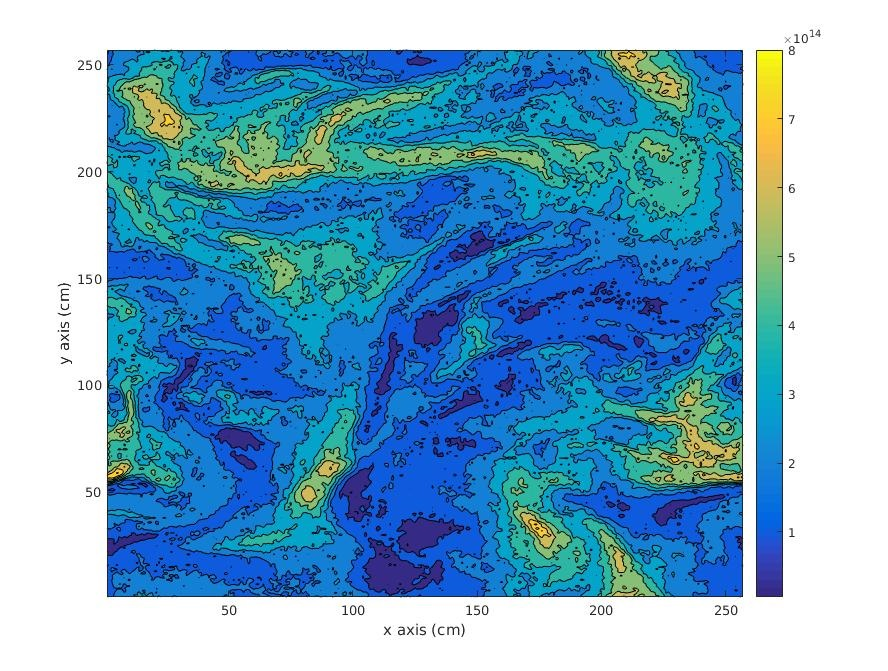
\includegraphics[width=9.5cm]{current_density_magnitude_slice.jpg}
\label{figure2}
\centering
\end{figure}
\vspace{.4cm}

These visualizations demonstrate the magnitudes and gradients of key components in defining energy within the simulation. Creating visual representations of the components of a systems energy and alignment are important because visuals allow for recognition of dramatic trends in simulation behavior which can be more opaque when only considering quantitative representations of datasets. Additionally, key structures and orientations can be recognized for possible discussion. Visible in the above plot are elongated strands of continuous current density magnitude, which are associated with the formation of filament substructures, a kind of structure responsible for dissipation whose orientation may be indicative of the system’s driving forces. The discussion of these structures led to an investigation of dynamic alignment, as the orientation of the bulk flow of particles with the net magnetic field is of some significance in modern plasma turbulence research \cite{boldyrev}. 

\vspace{.4cm}
\section{Dynamic Alignment}
\vspace{.4cm}

The investigation of dynamic aligment has become a notable trend in contemporary plasma turbulence research\cite{boldyrev2}, and has been instrumental in the modification of theory that attempts to apply plasma physics to astrophysics\cite{goldreich}. Because of this relevance, correlation was investigated between the velocity of plasma and the magnetic field in the simulation. The purpose of this investigation was to isolate trends that supported previous assertions\cite{boldyrev} regarding the orientation of bulk particle motion and the direction of the local magnetic field. Dynamic alignment is the theory that turbulent magnetic and velocity fluctuations become increasingly aligned at smaller scales, changing the nature of the MHD cascade. Physically, the change in bulk motion of particles will occur increasingly in the same direction as the change in local magnetic field as kinetic and electromagnetic behavior is observed in turbulent eddies of progressively lesser size. The mathematical description of this phenomenon is as follows, with $\vec{v}$ and $\vec{B}$ indicating fluid velocity and magnetic field, as previously.

\vspace{.1cm}
\begin{equation}
\theta=\arcsin[\frac{<|\Delta \vec{v} \times \Delta \vec{B}|>}{<|\Delta \vec{v}||\Delta \vec{b}|>}]
\label{equation3}
\end{equation}
\vspace{.1cm}

In the previous equation [Equation \eqref{equation3}], $\Delta$ indicates the presence of a cell separation $\delta x$ between locations $i$ and $j$ on the lattice, the difference between said values being what is entered into the above expression, as follows:

\vspace{.1cm}
\begin{equation}
\Delta \vec{v}=\vec{v}_j-\vec{v}_i
\label{equation4}
\end{equation}
{\centering (where $j-i=\delta x$)\\}
\vspace{.6cm}

The result of this investigation showed that discrepancies exist between the predictions of dynamic alignment trends and what is observed in simulation. By plotting the scale variant theta defined above, comparisons can be made between a random Gaussian distribution of data and the field created by the plasma simulations. In the theory of dynamic alignment, $\theta \propto \delta x^\alpha$, where $\alpha$ is an index which describes the rate of alignment. Below is an example of the theta given by both the simulation data and a dataset with random distribution [Fig. \ref{figure3}].

\vspace{.4cm}
\begin{figure}[H]
\caption{Dynamic Alignment Comparison of Simulation and Random Field}
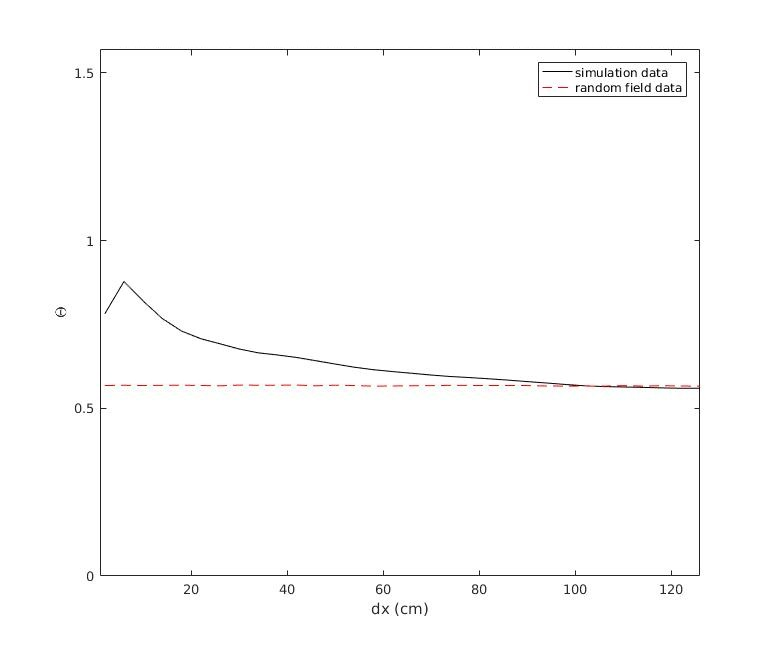
\includegraphics[width=9.5cm]{dynamicalignment.jpg}
\label{figure3}
\centering
\end{figure}


Above, the large scale value of dynamic alignment is demonstrated to be very similar to the behavior of random data, with a mean deviation of aproximately $3.1^{\circ}$ ($0.054$ radians) with a maximum observed $\theta$ of $50.3^{\circ}$ ($.878$ radians). This alignment increases with smaller $\delta x$, counter to the trend predicted in Boldyrev's 2005 \textit{On the Spectrum of Magnetohydrodynamic Turbulence} \cite{boldyrev2}. This disruption of alignment in contrast to MHD literature may be due to additional physics present in these simulations, including kinetic physics\cite{zhdankin}, relativistic effects, and limited inertial range.

Scale dependence was investigated in order to allow for connections to be made between the impact of dynamic alignment and the energy behavior of the system at different scales, which is an especially important characteristic of simulations such as this, which fundamentally involve energy transfer across a given range of scales.
 
\vspace{.4cm}
\section{Individual Particle Analysis}
\vspace{.4cm}

As a continuation of studying simulation behavior at progressively smaller scales, the final dataset investigated dealt directly with the behavior of individual particles. The statistical description of particle trajectories with respect to the native magnetic fields could provide further insight into dynamic alignment. It is vital to mention that the data used to analyze the behavior of individual particles in simulation is different from data previously discussed because the individual particle data describes particle movement over a cube with $1024^3$ volume, as opposed to the previously examined $256^3$ cell volume. All other parameters of the particle trajectory simulations are identical to their counterparts, which were discussed in the previous sections. For consistency, the foundation of this approach was the creation of visualizations of the overall trajectory of a given particle, then the isolation and description of finer features in the plot. An example of this is as follows. First, a projection of a particle's path onto the XY plane is plotted [Fig. \ref{figure4}].


\begin{figure}[H]
\caption{x-y Plane Projection of Selected Particle Trajectory}
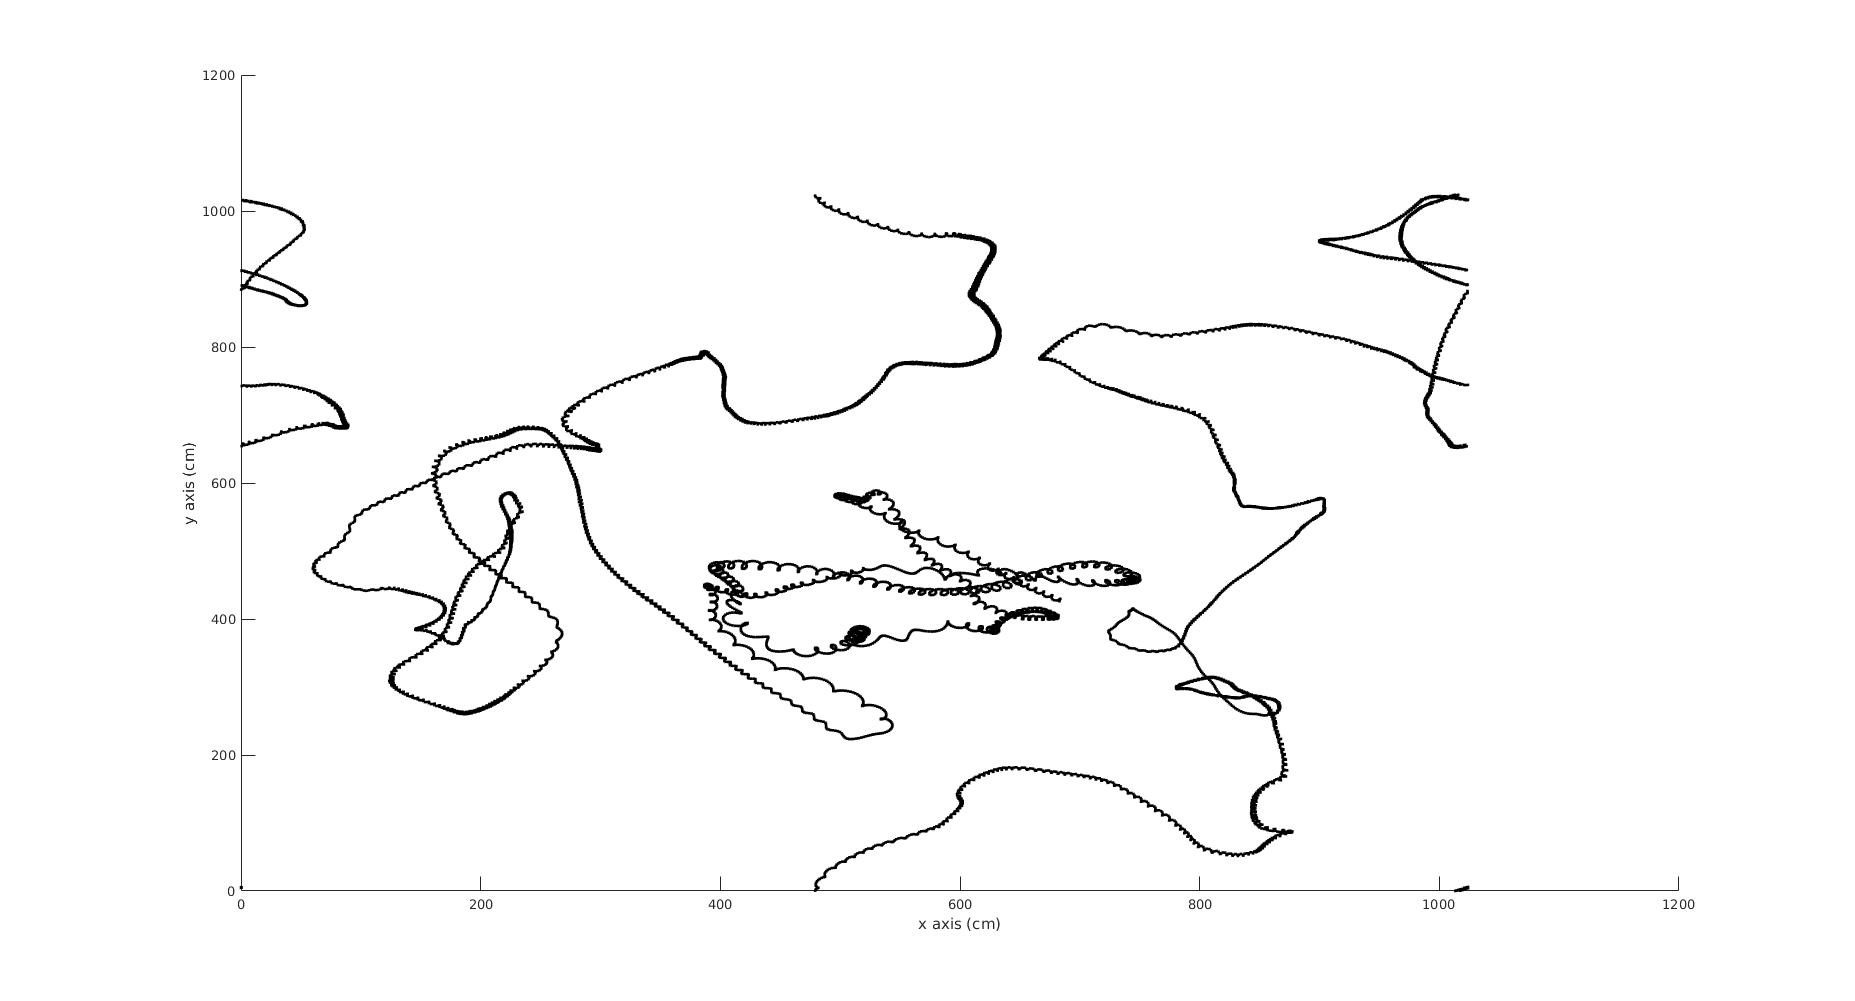
\includegraphics[width=10cm]{representative_2d_particle_trajectory.jpg}
\label{figure4}
\centering
\end{figure}

The movement of the particle over very short ranges can be identified as a tight oscillation circumscribing a larger trend in motion. In order to investigate the tight spiraling seen near the center of the above plot, the center of the previous plot was rendered in a 3D visualization \ref{figure5} in order to isolate description of the path in the same way that filament structures were described in the previous section.

\vspace{.4cm}
\begin{figure}[H]
\caption{3D Rendering of particle trajectory}
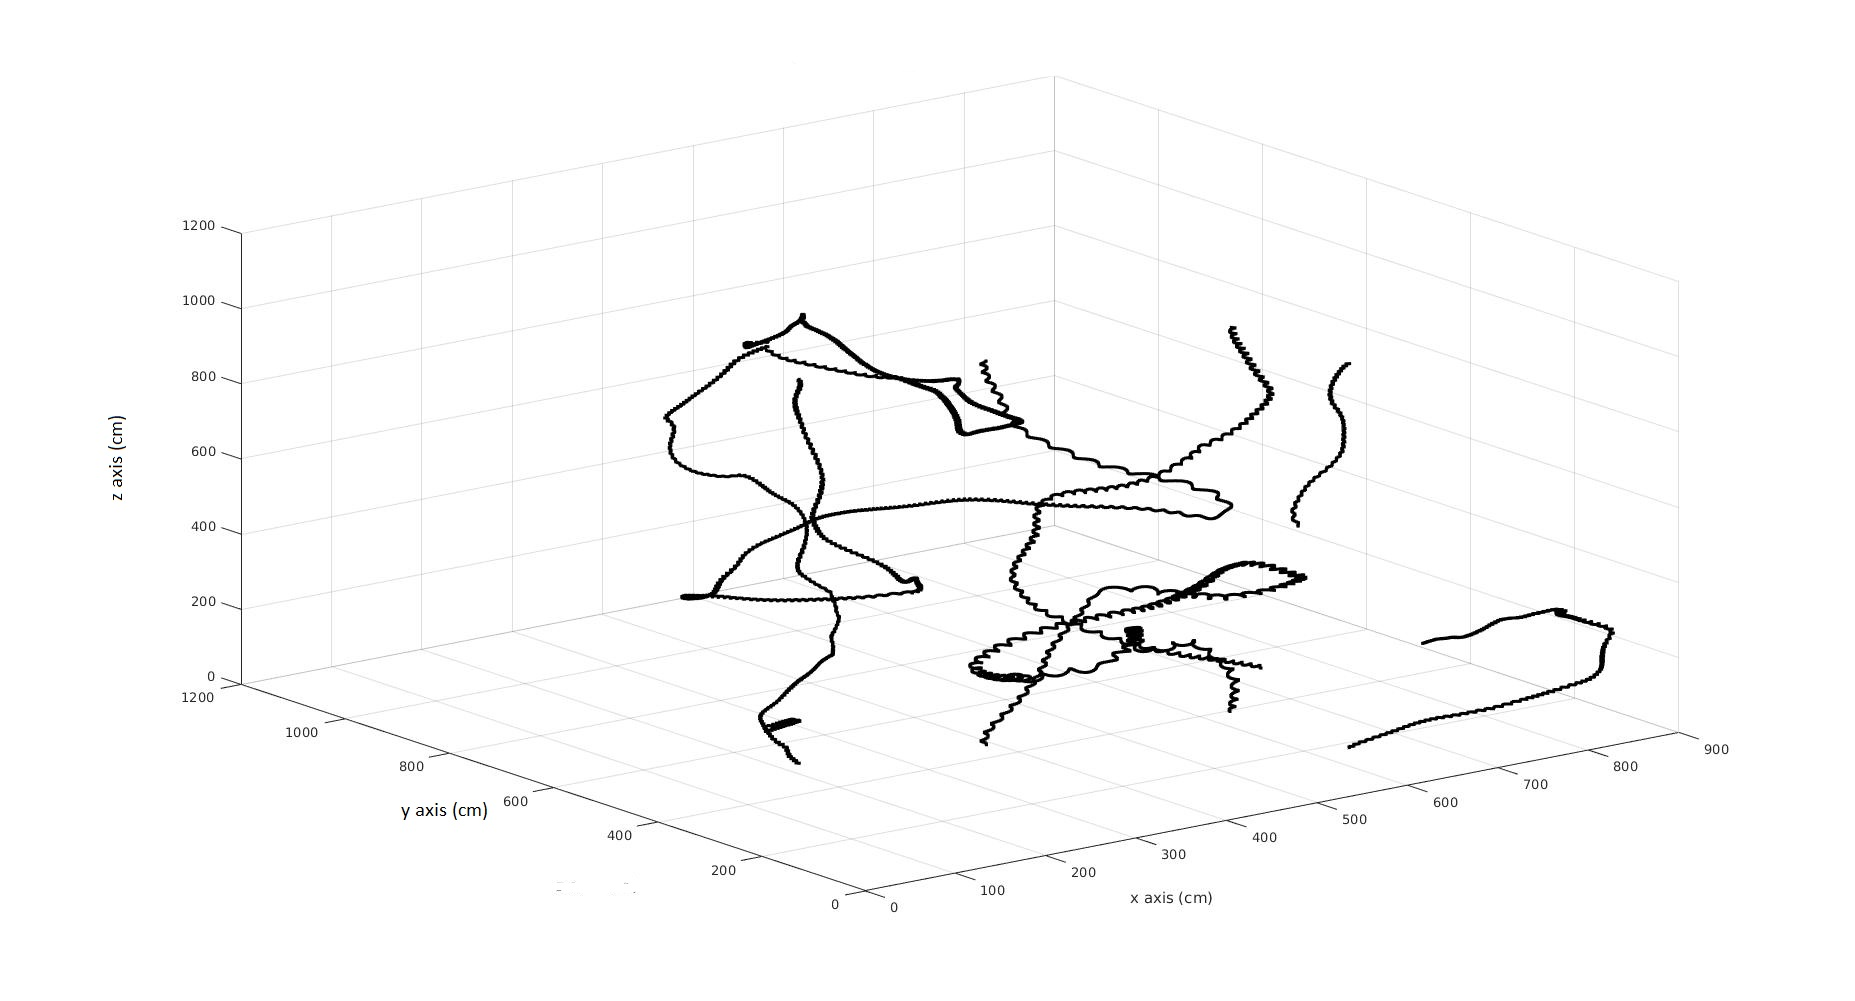
\includegraphics[width=10cm]{3d_plot_of_particle_trajectory_subset.jpg}
\label{figure5}
\centering
\vspace{.4cm}
\end{figure}

The presence of distinctly tight spirals in the particle trajectory is not surprising, however the instances observed of deflection of the tight spiraled motion is dramatic, and the localization of the tight spiraling indicates that observation of individual particles might lead to evidence of the local influence of dynamic alignment, which would help to clarify the assertions regarding dynamic alignment made previously. Additionally worth investigating are discrepancies between individual particle accelerations and what behavior is predicted by alignment with existing electric fields.

\vspace{.4cm}
\section{Conclusion}
\vspace{.4cm}

	Accompanied by readings from Biskamp\cite{biskamp} and associated plasma turbulence literature\cite{boldyrev}\cite{chandran}, visualizations of simulation components were used to identify critical structures formed by turbulence in a plasma body. Notably, these readings and associated discussions became focused on the simulation components associated with the Lorentz force. These components in turn led to an interest in the role of dynamic alignment in the simulations. To investigate this correlation of simulation components, particularly particle velocity and local magnetic field, were made at different scales to locate discrepancies from prediction. The resulting dynamic alignment at large scales was similar to a random field with gaussian distribution of values. To demonstrate the similarities a figure showing both trends [Fig. \ref{figure3}] was created, demonstrating visually the mean deviation of approximately $3.1^{\circ}$, ($0.054$ radians) between the two trends. The maximum observed $\theta$ of $50.3^{\circ}$ ($.878$ radians) shows that rather than becoming aligned, fluctuations tend to become more perpendicular to each other at small scales, which is the converse of the predictions in Boldyrev's 2005 \textit{On the Spectrum of Magnetohydrodynamic Turbulence} \cite{boldyrev2}.
A recommended extension of this study is the investigation of the relationship between individual particle trajectories and dynamic alignment. This should be conducted with focus on explaining why no scale dependence is observed in dynamic alignment and whether the trends observed in this paper and further particle trajectory observations are reflected in longer simulations, as well as time evolved simulations.

% Now we need a bibliography:
\begin{thebibliography}{9}

\bibitem{biskamp}
Biskamp, Dieter
\textit{Magnetohydrodynamic Turbulence}
Cambridge Univ Pr, 2009.
\vspace{.3cm}

\bibitem{boldyrev2}
Boldyrev, Stanislav
\textit{On the Spectrum of Magnetohydrodynamic Turbulence} 
The Astrophysical Journal, vol. 626, no. 1, 2005, doi:10.1086/431649.
\vspace{.3cm}

\bibitem{chandran}
Chandran, B. D. G., et al. 
\textit{Intermittency And Alignment In Strong Rmhd Turbulence.} 
The Astrophysical Journal, vol. 807, no. 1, 2015, p. 39., doi:10.1088/0004-637x/807/1/39.
\vspace{.3cm}

\bibitem{goldreich}
Goldreich, P., and S. Sridhar.
\textit{Toward a Theory of Interstellar Turbulence. 2: Strong Alfvenic Turbulence} 
The Astrophysical Journal, vol. 438, 1995, p. 763., doi:10.1086/175121.
\vspace{.3cm}

\bibitem{boldyrev}
Mason, Joanne, et al.
\textit{Dynamic Alignment in Driven Magnetohydrodynamic Turbulence}
Physical Review Letters, vol. 97, no. 25, 2006, doi:10.1103/physrevlett.97.255002.
\vspace{.3cm}

\bibitem{zhdankin}
Zhdankin, Vladimir, et al.
\textit{Kinetic Turbulence in Relativistic Plasma: From Thermal Bath to Nonthermal Continuum.}
Physical Review Letters, vol. 118, no. 5, Mar. 2017, doi:10.1103/physrevlett.118.055103.



\end{thebibliography}

\end{document}